\documentclass[]{tufte-handout}

% ams
\usepackage{amssymb,amsmath}

\usepackage{ifxetex,ifluatex}
\usepackage{fixltx2e} % provides \textsubscript
\ifnum 0\ifxetex 1\fi\ifluatex 1\fi=0 % if pdftex
  \usepackage[T1]{fontenc}
  \usepackage[utf8]{inputenc}
\else % if luatex or xelatex
  \makeatletter
  \@ifpackageloaded{fontspec}{}{\usepackage{fontspec}}
  \makeatother
  \defaultfontfeatures{Ligatures=TeX,Scale=MatchLowercase}
  \makeatletter
  \@ifpackageloaded{soul}{
     \renewcommand\allcapsspacing[1]{{\addfontfeature{LetterSpace=15}#1}}
     \renewcommand\smallcapsspacing[1]{{\addfontfeature{LetterSpace=10}#1}}
   }{}
  \makeatother

\fi

% graphix
\usepackage{graphicx}
\setkeys{Gin}{width=\linewidth,totalheight=\textheight,keepaspectratio}

% booktabs
\usepackage{booktabs}

% url
\usepackage{url}

% hyperref
\usepackage{hyperref}

% units.
\usepackage{units}


\setcounter{secnumdepth}{-1}

% citations

% pandoc syntax highlighting

% longtable

% multiplecol
\usepackage{multicol}

% strikeout
\usepackage[normalem]{ulem}

% morefloats
\usepackage{morefloats}


% tightlist macro required by pandoc >= 1.14
\providecommand{\tightlist}{%
  \setlength{\itemsep}{0pt}\setlength{\parskip}{0pt}}

% title / author / date
\date{}


\begin{document}





\thispagestyle{empty}

\noindent\LARGE \emph{Andrew and Tom Meyer Property}\\
\noindent\Large \emph{Forest Management Plan}\\
\noindent\Large \emph{July 09, 2020}

\normalsize 

\begin{marginfigure}
\hspace{2pt}\newline\vspace{80pt}
\noindent \textit{\large Effective date of plan}  
\newline\indent April 1, 2020  
\end{marginfigure}

\begin{marginfigure}
\noindent \textit{\large Property}   
\newline\indent 91.45 acres    
\newline\indent Hardwick, VT  
\newline\indent SPAN 282-089-11700  
\newline\indent Mapping based on VMP photo(s)  
\newline\indent 160220, 160224, 164220, 164224  
\end{marginfigure}

\begin{marginfigure}
\noindent \textit{\large Owner}
\newline\indent Andrew and Thomas Meyer  
\newline\indent 3707 Bridgman Hill Road
\indent 
\newline\indent Hardwick, VT 05843  
\end{marginfigure}

\begin{marginfigure}
\noindent \textit{\large Prepared by} 
\newline\indent Neal F. Maker and John D. Foppert  
\newline\indent Pekin Branch Forestry  
\newline\indent 1324 West County Road  
\newline\indent Calais, VT 05648  
\newline\indent (802) 229-9757  
\vspace{100pt}\end{marginfigure}

\vspace{30pt} \indent This forest management plan is a blueprint for
responsible land stewardship. It is the result of a planning process
that incorporated an assessment of the history and current conditions on
the property, consideration of the various courses of future development
that the forest could follow, and discernment as to which outcomes best
suit the landowners' particular objectives.

\vspace{20pt} By signing below, I certify that I approve of---and agree
to manage my forestland according to---the following management plan. I
further certify that any of my forestland that is enrolled in Vermont's
Use Value Appraisal program is under active long-term forest management
in accordance with the state's minimum acceptable standards for forest
management. These standards include following Acceptable Management
Practices to maintain water quality on logging operations.

\vspace{22pt}

\noindent\rule{7.3cm}{0.4pt} \rule{.3cm}{0pt} \rule{3cm}{0.4pt}

\noindent Landowner \rule{6cm}{0pt} Date

\vspace{18pt}

\noindent\rule{7.3cm}{0.4pt} \rule{.3cm}{0pt} \rule{3cm}{0.4pt}

\noindent Landowner \rule{6cm}{0pt} Date

\vspace{18pt}

\noindent\rule{7.3cm}{0.4pt} \rule{.3cm}{0pt} \rule{3cm}{0.4pt}

\noindent Landowner \rule{6cm}{0pt} Date

\vspace{18pt}

\noindent\rule{7.3cm}{0.4pt} \rule{.3cm}{0pt} \rule{3cm}{0.4pt}

\noindent Landowner \rule{6cm}{0pt} Date

\begin{marginfigure}

{\centering 
\includegraphics[width=0.9\linewidth,height=0.9\textheight]{C:/Users/Neal/projects/cruise/logo-small-gray80} 

}

\end{marginfigure}

\vspace{35pt}

This forest management plan meets the standards promulgated by the
Vermont Department of Forests, Parks and Recreation as required for
eligibility in the Use Value Appraisal Program.

\vspace{22pt}

\noindent\rule{7.3cm}{0.4pt} \rule{.3cm}{0pt} \rule{3cm}{0.4pt}

\noindent County Forester \rule{5.3cm}{0pt} Date

\pagebreak

\section{Introduction}\label{introduction}

This plan covers the ten year period from 2021 to 2030. It lays out the
near- and medium-term actions that should guide the development of the
Andrew and Tom Meyer Forest. It also qualifies the property for Use
Value Appraisal (UVA) and commensurate reduction in property
taxes.\footnote{Further information about UVA and current valuations can
  be found at the Vermont Tax Department's website:
  \url{https://tax.vermont.gov/property-owners/current-use}.
  \vspace{20pt}} Owners participating in the Use Value Appraisal program
are obliged to manage their property according to the plan and to make
any reasonable investments for improvement that the plan
recommends.\footnote{UVA management plan standards are determined by the
  Department of Forests, Parks, \& Recreation and are available at
  \url{https://fpr.vermont.gov/forest/your_woods/use_value_appraisal} or
  through a County Forester.}

The plan is organized to reflect the forest decision making process. It
begins with a general overview of the property, then lays out the
landowner's management goals, before exploring the forest in detail and
discussing the actions that could be taken to help meet those goals. Its
recommendations were developed in accordance with the principles and
practices of scientifically sound forestry, as described in the relevant
management guidelines, textbooks and academic journals.

\section{Property Description}\label{property-description}

Some 84 percent of the 91.45 acre Andrew and Tom Meyer property is
productive forestland that will be managed according to this plan. Its
elevations range from 1140 to 1270 feet above mean sea level. One
unnamed stream flows south across the property and into the Lamoille
River in Hardwick. A small open wetland borders the stream as well, and
accounts for all of the property's non-productive forestland. The stream
and marsh limit vehicular access somewhat, but the great majority of the
property's forestland is easily reached on a network of existing trails,
which connect to a recently constructed access off Center Road. Property
boundaries are demarcated by old flagging and healed over blazes, many
of which have been repainted blue. The lines can be difficult to locate,
and should be re-flagged before any logging operations. Soils, forest
health, and other pertinent topics are discussed in the individual stand
area descriptions that follow.

\section{Principles, Goals \& Strategies For Forest
Management}\label{principles-goals-strategies-for-forest-management}

The following sections describe the chief principles and goals that
should guide forest management on the property; and outline the general
strategies that can be used to support them.

\begin{marginfigure}

{\centering 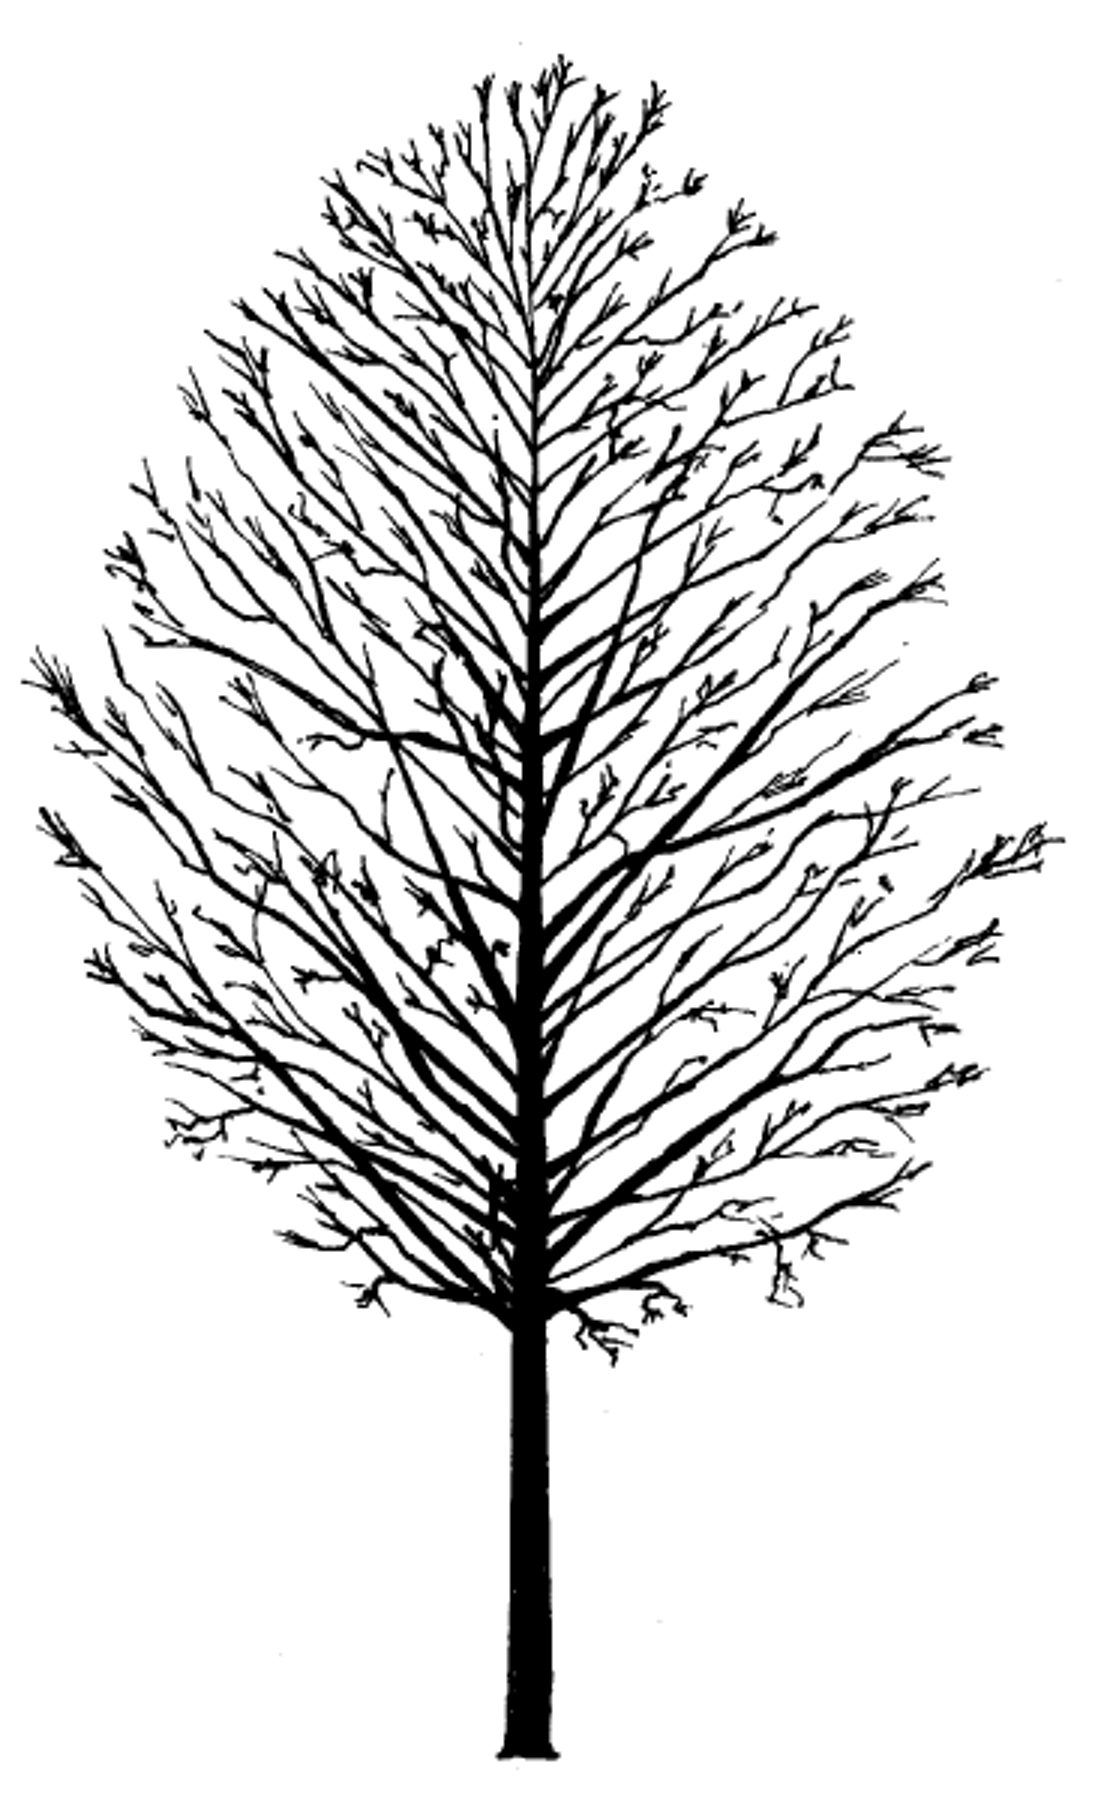
\includegraphics[width=0.7\linewidth,height=0.7\textheight]{C:/Users/Neal/projects/cruise/maple} 

}

\end{marginfigure}

\subsection{Conservation}\label{conservation}

The ecological functioning, productive capacity and biological diversity
of the forest resource should be maintained or improved over time so as
to provide opportunities for the current or future landowners to
continue to enjoy and use the property. A management strategy that is
sustainable in the long-term and viable in the short- and medium-terms
offers a strong measure of protection against future development or
conversion.

\subsection{Ecological integrity, wildlife habitat, and
biodiversity}\label{ecological-integrity-wildlife-habitat-and-biodiversity}

Management should prioritize the protection of critical ecological
functions, water resources, and threatened or rare plant and wildlife
communities. Wetlands and stream-side riparian zones should be carefully
delineated and protected; and management should give consideration to
the habitat needs of native wildlife populations and to the relationship
between the property, its neighbors and the larger landscape they are
nested within. Management should be informed by and aim to improve
landscape diversity, wildlife travel corridors, and habitat
connectivity. Locally under-represented habitat types should be
identified and promoted. Stand scale and sub-stand scale management
should focus on developing or maintaining species-specific habitat
needs, such as nesting sites, cover, mast production, preferred browse
or other unique structural and compositional requirements.

\subsection{Timber management}\label{timber-management}

Management should provide regular returns from timber harvesting.
Long-term value growth is provided by maintaining full site occupancy
with healthy trees capable of producing high quality sawtimber or
veneer. Tree species which yield sought-after, high-value wood should be
promoted within each stand or, when regenerating a new stand, attention
should be paid to creating stand conditions that favor the establishment
of those species. At a property-wide scale, a variety of species should
be maintained, providing options for seizing future market opportunities
and a hedge against species-specific market depreciation. Among desired
species, additional preference should be given to individual trees of
sufficient vigor and grade-potential for strong future value growth.
Consideration of economic efficiency should inform the timing and
coordination of infrastructure investments and stand maintenance,
improvement and harvest operations.

\subsection{Scenery, recreation, and
exploration}\label{scenery-recreation-and-exploration}

Conscientious management can create or maintain a landscape that is
attractive, accessible and conducive to reflection, exploration and
appreciation. Attractiveness can be managed for by fostering diversity
within the landscape: accelerating the growth and development of the
most receptive individual trees in some places; maintaining the look,
feel and accompanying privacy provided by a dense forest in other
places; and elsewhere creating occasional vistas out from the forest and
improvements in depth of visual penetration within it. Attentive
maintenance of existing roads and trails and thoughtful improvements to
the trail network should facilitate the satisfying use of the property,
creating an appropriate balance between access and connectedness, on the
one hand, while preserving places of refuge and sanctuary, on the other.
A system of roads and trails of various sizes, suited for various
purposes, and interconnected with a broader trail network, provide for
both enjoyable recreation and efficient operations. An inviting, easily
accessed working forest should also encourage study and intellectual
exploration, allowing an interested land owner to become increasingly
knowledgeable about their land and positioned to contribute meaningfully
to its ongoing management.

\section{Stand Descriptions \& Management
Recommendations}\label{stand-descriptions-management-recommendations}

\begin{marginfigure} \noindent \textit{\LARGE Management Schedule} 

 \vspace{10 pt} 

 \noindent \textit{\large 2024} 

 \begin{itemize} \item Area 1: Single tree selection 

 \end{itemize} \vspace{10 pt} 

 \noindent \textit{\large 2029} 

 \begin{itemize} \item Reinventory forest 

 \end{itemize} \end{marginfigure}

Presented below are detailed stand-by-stand descriptions of the forest,
the long-term structural, compositional and functional goals for each
stand, and the near-term silvicultural treatments or management
activities that have been prescribed to advance each stand toward those
goals. The data presented in the following pages was obtained from a
field examination of the property in July of 2020. General conditions
were assessed qualitatively in conjunction with quantitative sampling.
Observational notes and sample summary statistics together provide the
basis for the area descriptions and management recommendations. All
sampling was done using a systematic sample and variable radius plots.
In stands with uneven-aged structures, all trees 6" dbh and larger were
measured in each plot. In stands with even-aged structures, all
main-canopy trees were measured in each plot.

When contractors are used to implement silvicultural prescriptions, they
should be highly skilled, properly equipped, fully insured, and closely
supervised. A professional forester should prepare and administer
commercial treatments, and logging operations should be timed to
coincide with favorable weather conditions (working on wet soils only
when they are frozen, for instance) and favorable timber markets. Use
Value Appraisal program guidelines allow any management activities
prescribed in this plan to be carried out up to three years before or
after the date indicated. Landowners in the Use Value Appraisal program
must file a Forest Management Activity Report with the County Forester
by February 1\textsuperscript{st} if any commercial logging occurred in
the previous year.

The property should be reinventoried in 2029 and the findings brought to
bear on a reassessment of the goals and strategies proposed in this
plan, leading to a formal management plan update. At any point over the
course of this management period, this plan may be updated to
incorporate new information and to reflect any new thoughts, concerns or
considerations on the part of the landowner or the foresters helping to
manage the land.

\newpage

\section{Area 1}\label{area-1}

Mixed softwood\\
\noindent 63.33 legal acres \textbar{} 61.87 measured acres

\subsection{Site-specific information}\label{site-specific-information}

\begin{quote}
\begin{itemize}
\tightlist
\item
  \textbf{Soils:}\\
  \indent\indent  \textbf{Vershire-Lombard complex} (moderately deep,
  well drained, very stony glacial till on summits, shoulders, and
  backslopes)\\
  \textbf{Buckland silt loam} (very deep, moderately well drained, very
  stony dense glacial till on footslopes)\\
  \textbf{Cabot silt loam} (very deep, poorly drained, very stony dense
  glacial till on toeslopes and drainageways)
\end{itemize}
\end{quote}

\begin{quote}
\begin{itemize}
\tightlist
\item
  \textbf{Site Class:}\\
  \vspace{2pt} II -- III (determined from soil mapping and field
  assessment)
\end{itemize}
\end{quote}

\begin{quote}
\begin{itemize}
\tightlist
\item
  \textbf{Access:}\\
  \vspace{2pt} Good trail network with the potential to tie in to trails
  on nearby properties. All forestland is less than 1 mile from Center
  Road and a good access road was constructed off Center Road about a
  decade ago. Some wet areas in the south and west are better accessed
  on frozen soils.
\end{itemize}
\end{quote}

\begin{quote}
\begin{itemize}
\tightlist
\item
  \textbf{Stand history:}\\
  \vspace{2pt} History of periodic logging. Portions of the stand were
  logged in the early 90s, leading to variable stocking and age
  structures.
\end{itemize}
\end{quote}

\subsection{Current forest
information}\label{current-forest-information}

\begin{quote}
\begin{itemize}
\tightlist
\item
  \textbf{Age Class Structure:}\\
  \vspace{2pt} Uneven-aged\\

  \begin{marginfigure}
  \includegraphics{fmp-vt_files/figure-latex/unnamed-chunk-2-1} \caption[Distributions are approximated with kernel density estimation]{Distributions are approximated with kernel density estimation. Common species are those that account for at least 8 percent of the total stocking and areas under each curve represent species basal areas.}\label{fig:unnamed-chunk-2}
  \end{marginfigure}
\end{itemize}
\end{quote}

\begin{quote}
\begin{itemize}
\tightlist
\item
  \textbf{Average stocking (with 95\% confidence intervals):}\\
  \vspace{2pt} 141 sq ft basal area (+/- 28 sq ft)\\
  10.5" quadratic stand diameter (+/- 0.6``)\\
  234 trees per acre (+/- 48 trees)\\
  \vspace{8pt}
\end{itemize}
\end{quote}

\begin{tabular}{lrrrr}
\toprule
Size Class & Total & AGS & UGS & Target\\
\midrule
6-11 in. & 55 & 48 & 7 & 40\\
12-15 in. & 66 & 63 & 4 & 45\\
16-21 in. & 14 & 12 & 2 & 12\\
22+ in. & 6 & 4 & 1 & 0\\
Total & 141 & 127 & 14 & 97\\
\bottomrule
\end{tabular}

\vspace{2pt}
\footnotesize\parbox{200pt}{Current (total, acceptable, and unacceptable growing stock) and post-harvest target basal areas (sq ft/ac) by size class.}\normalsize

\begin{quote}
\begin{itemize}
\tightlist
\item
  \textbf{Species (\% stocking):}\\
  \vspace{2pt} cedar (21\%), spruce (21\%), hemlock (19\%), fir (9\%),
  soft maple (9\%), hard maple (5\%), white pine (4\%), aspen (4\%),
  paper birch (3\%), yellow birch (3\%), ash (2\%), black cherry (1\%),
  other hardwood (1\%), tamarack (1\%)
\end{itemize}
\end{quote}

\begin{quote}
\begin{itemize}
\tightlist
\item
  \textbf{Regeneration:}\\
  \vspace{2pt} Scattered fir, spruce and yellow birch in areas of higher
  stocking, where there was no logging in the 90s. Logged areas host
  abundant fir, spruce, paper birch, and yellow birch saplings,
  especially where stocking was brought below about 100 square feet.
\end{itemize}
\end{quote}

\begin{quote}
\begin{itemize}
\tightlist
\item
  \textbf{Forest health:}\\
  \vspace{2pt} Relatively high mortality in fir, even among poles. One
  non-native honeysuckle was observed during the inventory and removed.
  Invasive plants are not a threat, but should be watched for so that
  any developing populations can be kept in check. Heavy deer browse
  probably inhibited hardwood regeneration after the last logging
  operation and pushed the composition toward fir and spruce.
\end{itemize}
\end{quote}

\subsection{Inventory information}\label{inventory-information}

\begin{quote}
\begin{itemize}
\tightlist
\item
  14 points, 10 BAF, July, 2020
\end{itemize}
\end{quote}

\begin{figure}
\includegraphics{fmp-vt_files/figure-latex/unnamed-chunk-6-1} \caption[Points represent individual plots]{Points represent individual plots. Asterisk represnts stand average. Radial lines are quadratic stand diameters.}\label{fig:unnamed-chunk-6}
\end{figure}

\subsection{Long-term management
system}\label{long-term-management-system}

\textbf{Selection system}

We will continue to manage the stand using uneven-aged techniques.
Single tree selection has been the dominant paradigm in at least the
last several cutting cycles, and seems to be working. The last logging
operation covered about half of the stand area, left a healthy residual,
and triggered abundant regeneration. We plan to continue using single
tree selection treatments, with a 15 or 20 year cutting cycle, residual
basal areas of 80 to 100 square feet per acre (after Frank and Bjorkbom
\protect\hyperlink{ref-frank_silvicultural_1973}{1973}), and diameter
objectives that vary by species. Balsam fir and aspen should be
considered mature at 14'' dbh; spruce, red maple, black cherry, and
paper birch at 18''; and white pine, hard maple, and yellow birch at
20''. While cedar is well represented in the stand by basal area, it is
is mostly limited to denser `microstands' on wet soils within the larger
stand. These areas should not be treated the same as the rest of the
stand because high deer browse pressure will almost certainly prevent
the cedar from regenerating, and it will eventually be replaced by other
species. This process has been eroding cedar populations across the
northeastern US and eastern Canada for the last half century. Instead,
cedar pockets should be treated as even-aged inclusions until the deer
population is less or steps have been taken to prevent their browse. At
that time concerted efforts can be made to regenerate the next
generation of cedar with a reasonable chance of success. (See Larouche
and Ruel (\protect\hyperlink{ref-larouche_development_2015}{2015}) and
Boulfroy et al.
(\protect\hyperlink{ref-boulfroy_silvicultural_2012}{2012}) for more
information. )

\subsection{Silvicultural
prescription}\label{silvicultural-prescription}

\textbf{Single tree selection}\\
\noindent \textbf{Year:} 2024

The areas of the stand with higher stocking, that were not logged in the
90s, should be treated using single tree selection when softwood timber
markets become favorable. Generally, the basal area should be reduced to
80 or 100 square feet per acre (after Frank and Bjorkbom
\protect\hyperlink{ref-frank_silvicultural_1973}{1973}) with the goal of
meeting the post-harvest target basal areas by size class that are
presented in the diameter distribution table above (under ``Current
forest information''). This will allow us to simultaneously capture the
value of mature trees, thin immature cohorts, and establish a new
cohort. The residual species composition should generally reflect the
existing composition, though we expect to decrease the relative
abundance of fir and hemlock somewhat and increase the relative
abundance of spruce. Spruce, maple, and birch will ideally be
regenerated, but deer browse pressure will probably limit hardwood
regeneration and advance fir regeneration will persist. Tending in
future harvests can be used to decrease the fir component. Hunting in
the years after the treatment could also help to increase the survival
of hardwood regeneration. In areas dominated by cedar, the stocking
should be kept higher (perhaps 150 square feet per acre) and well formed
cedars with large crowns should be retained, to ensure that a healthy
cedar population will remain until cedar can be successfully
regenerated. \par Logging should either be carried out in winter on
frozen soils, or skid trails should be carefully located to keep
equipment out of wet areas. The treatment will also be a good
opportunity to improve the recreational trail network, and pre-harvest
skid trail layout will ensure that any new trails that are built will
contribute to the property's recreation potential.

\newpage

\section{Area 2}\label{area-2}

Northern hardwood\\
\noindent 13.16 legal acres \textbar{} 12.86 measured acres

\subsection{Site-specific
information}\label{site-specific-information-1}

\begin{quote}
\begin{itemize}
\tightlist
\item
  \textbf{Soils:}\\
  \indent\indent  \textbf{Vershire-Lombard complex} (moderately deep,
  well drained, very stony glacial till on summits, shoulders, and
  backslopes)\\
  \textbf{Buckland silt loam} (very deep, moderately well drained, very
  stony dense glacial till on footslopes)
\end{itemize}
\end{quote}

\begin{quote}
\begin{itemize}
\tightlist
\item
  \textbf{Site Class:}\\
  \vspace{2pt} II -- III (determined from soil mapping and field
  assessment)
\end{itemize}
\end{quote}

\begin{quote}
\begin{itemize}
\tightlist
\item
  \textbf{Access:}\\
  \vspace{2pt} Good trail network. All forestland is less than 1 mile
  from Center Road. Wet area in the east should be avoided until trees
  have fully established themselves.
\end{itemize}
\end{quote}

\begin{quote}
\begin{itemize}
\tightlist
\item
  \textbf{Stand history:}\\
  \vspace{2pt} Developed from abandoned pasture c. 1960s. Much of the
  stand established well and is now in the stem exclusion phase of
  development; but wetter soils in the east, near Center road, have
  delayed establishment and left areas dominated by herbaceous growth.
  We suspect that this wet area will develop a closed canopy eventually,
  but probably not in the next several decades.
\end{itemize}
\end{quote}

\subsection{Current forest
information}\label{current-forest-information-1}

\begin{quote}
\begin{itemize}
\tightlist
\item
  \textbf{Age Class Structure:}\\
  \vspace{2pt} Even-aged\\

  \begin{marginfigure}
  \includegraphics{fmp-vt_files/figure-latex/unnamed-chunk-7-1} \caption[Distributions are approximated with kernel density estimation]{Distributions are approximated with kernel density estimation. Common species are those that account for at least 8 percent of the total stocking and areas under each curve represent species basal areas.}\label{fig:unnamed-chunk-7}
  \end{marginfigure}
\end{itemize}
\end{quote}

\begin{quote}
\begin{itemize}
\tightlist
\item
  \textbf{Average stocking (with 95\% confidence intervals):}\\
  \vspace{2pt} 75 sq ft basal area (+/- 49 sq ft)\\
  6.2" quadratic stand diameter (+/- 1.9``)\\
  356 trees per acre (+/- 244 trees)\\
  \vspace{8pt}
\end{itemize}
\end{quote}

\begin{tabular}{lrrr}
\toprule
Size Class & Total & AGS & UGS\\
\midrule
6-11 in. & 58 & 48 & 10\\
12-15 in. & 8 & 8 & 0\\
16-21 in. & 0 & 0 & 0\\
22+ in. & 0 & 0 & 0\\
Total & 65 & 55 & 10\\
\bottomrule
\end{tabular}

\vspace{2pt}
\footnotesize\parbox{200pt}{Current basal area (sq ft/ac) of total growing stock, acceptable growing stock (AGS), and unacceptable growing stock (UGS) by size class.}\normalsize

\begin{quote}
\begin{itemize}
\tightlist
\item
  \textbf{Species (\% stocking):}\\
  \vspace{2pt} soft maple (54\%), hard maple (12\%), aspen (8\%), fir
  (8\%), yellow birch (8\%), ash (4\%), black cherry (4\%), cedar (4\%)
\end{itemize}
\end{quote}

\begin{quote}
\begin{itemize}
\tightlist
\item
  \textbf{Regeneration:}\\
  \vspace{2pt} Young stand is still in stand establishment and stem
  exclusion phases, and has not developed any advance regeneration.
\end{itemize}
\end{quote}

\begin{quote}
\begin{itemize}
\tightlist
\item
  \textbf{Forest health:}\\
  \vspace{2pt} A couple of exotic honeysuckle plants were observed in
  the wet open area, but they only constitute a very minor infestation
  and should not be a problem as long as machinery is excluded.
\end{itemize}
\end{quote}

\subsection{Inventory information}\label{inventory-information-1}

\begin{quote}
\begin{itemize}
\tightlist
\item
  4 points, 10 BAF, July, 2020
\end{itemize}
\end{quote}

\begin{figure}
\includegraphics{fmp-vt_files/figure-latex/unnamed-chunk-11-1} \caption[Points represent individual plots]{Points represent individual plots. Asterisk represnts stand average. Radial lines are quadratic stand diameters.}\label{fig:unnamed-chunk-11}
\end{figure}

\subsection{Long-term management
system}\label{long-term-management-system-1}

\textbf{Even-aged management}

This stand should be managed using even-aged techniques and grown on a
rotation of about 100 years. We believe the stand is 50 or 60 years old
now. Thinnings should be carried out every 15 or 20 years, starting when
trees reach merchantable sizes.

\subsection{Silvicultural
prescription}\label{silvicultural-prescription-1}

No logging is necessary in this young stand over the next ten years.
Efforts to eradicate honeysuckle from the wet, eastern section of the
stand could pay off, though they don't appear to be spreading. At the
least, they should be monitored so they can be dealt with if they do
begin to spread. Wet-tolerant trees could be planted in open spots too,
to speed stand establishment, but planting is not necessary.

\newpage

\section{References}\label{references}

\setlength{\parindent}{0pt} \setlength{\parskip}{1.5em}

\hypertarget{refs}{}
\hypertarget{ref-boulfroy_silvicultural_2012}{}
Boulfroy, Emmanuelle, Eric Forget, Philip V. Hofmeyer, Laura S. Kenefic,
Catherine Larouche, Guy Lessard, Jean-Martin Lussier, Fred Pinto,
Jean-Claude Ruel, and Aaron. Weiskittel. 2012. ``Silvicultural Guide for
Northern White-Cedar (Eastern White Cedar).'' NRS-GTR-98. Newtown
Square, PA: U.S. Department of Agriculture, Forest Service, Northern
Research Station.
doi:\href{https://doi.org/10.2737/NRS-GTR-98}{10.2737/NRS-GTR-98}.

\hypertarget{ref-frank_silvicultural_1973}{}
Frank, Robert M., and John C. Bjorkbom. 1973. ``A Silvicultural Guide
for Spruce-Fir in the Northeast.'' Gen. Tech. Rep. NE-6. USDA FS
Northeastern Experiment Station.

\hypertarget{ref-larouche_development_2015}{}
Larouche, Catherine, and Jean-Claude Ruel. 2015. ``Development of
Northern White-Cedar Regeneration Following Partial Cutting, with and
Without Deer Browsing.'' \emph{Forests} 6 (12): 344--59.
doi:\href{https://doi.org/10.3390/f6020344}{10.3390/f6020344}.



\end{document}
